Pour le déplacement des capsules de leur plaque jusqu'aux réacteurs, trois idées ont été étudiées : 
\begin{itemize}
    \item Transport pneumatique par tube,
    \item convoyeur,
    \item robot 
\end{itemize}
\subsection*{Transport pneumatique par tube}
Le système de transport pneumatique par tube, serait de tuyaux dans lesquelles navigue les microcapsules grâce à une différence de pression de chaque coté de la microcapsule. Ce système est déja présent dans les hôpitaux et dans les grandes surfaces.
\begin{figure}[h!]
    \centering
    \begin{subfigure}{0.45\textwidth}
        \centering
        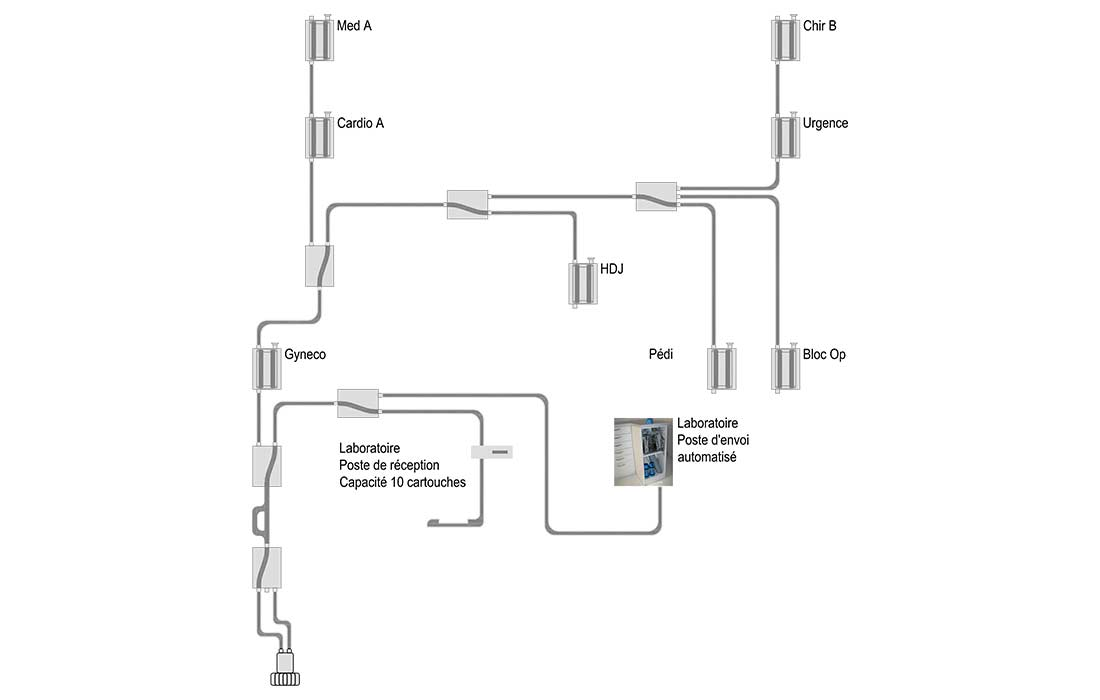
\includegraphics[width=\linewidth]{assets/figures/Hardware/transport_pneu/reseau_pneumatique_hopital.jpg} % Remplacez par le chemin de votre première image
        \caption{Schéma d'un réseau de transport pneumatique}
    \end{subfigure}\hfill
    \begin{subfigure}{0.45\textwidth}
        \centering
        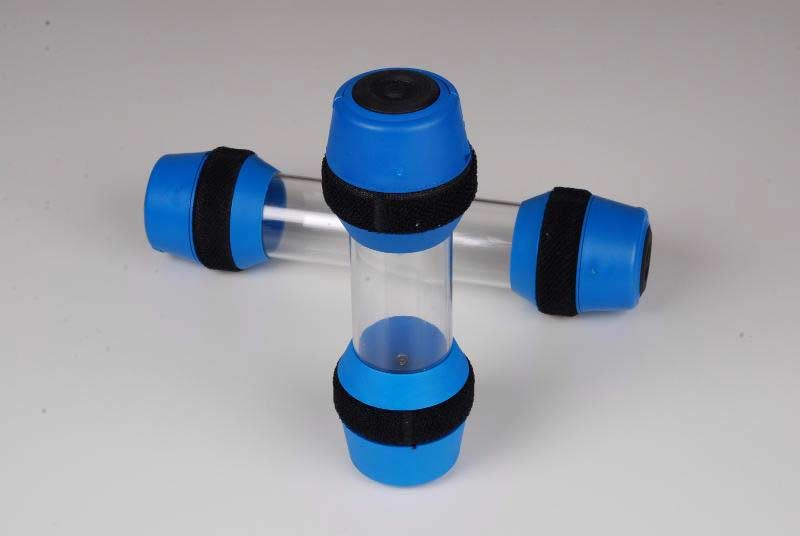
\includegraphics[width=\linewidth]{assets/figures/Hardware/transport_pneu/cartouche_transport_pneu.jpg} % Remplacez par le chemin de votre seconde image
        \caption{Cartouche pneumatique}
    \end{subfigure}
    \caption{Exemples de réseau de transport pneumatique par tube}
\end{figure}

\subsection*{Transport par convoyeur}
Pour déplacer les microcapsules, un convoyeur peut être utilisé, il faut néanmoins que le convoyeur soit adapter au microcapsule, un convoyeur à bande lisse ne fonctionnerais donc pas, mais une bande à tasseau ou un demi tube conviendrais parfaitement.
\begin{figure}[h!]
    \centering
    \begin{subfigure}{0.45\textwidth}
        \centering
        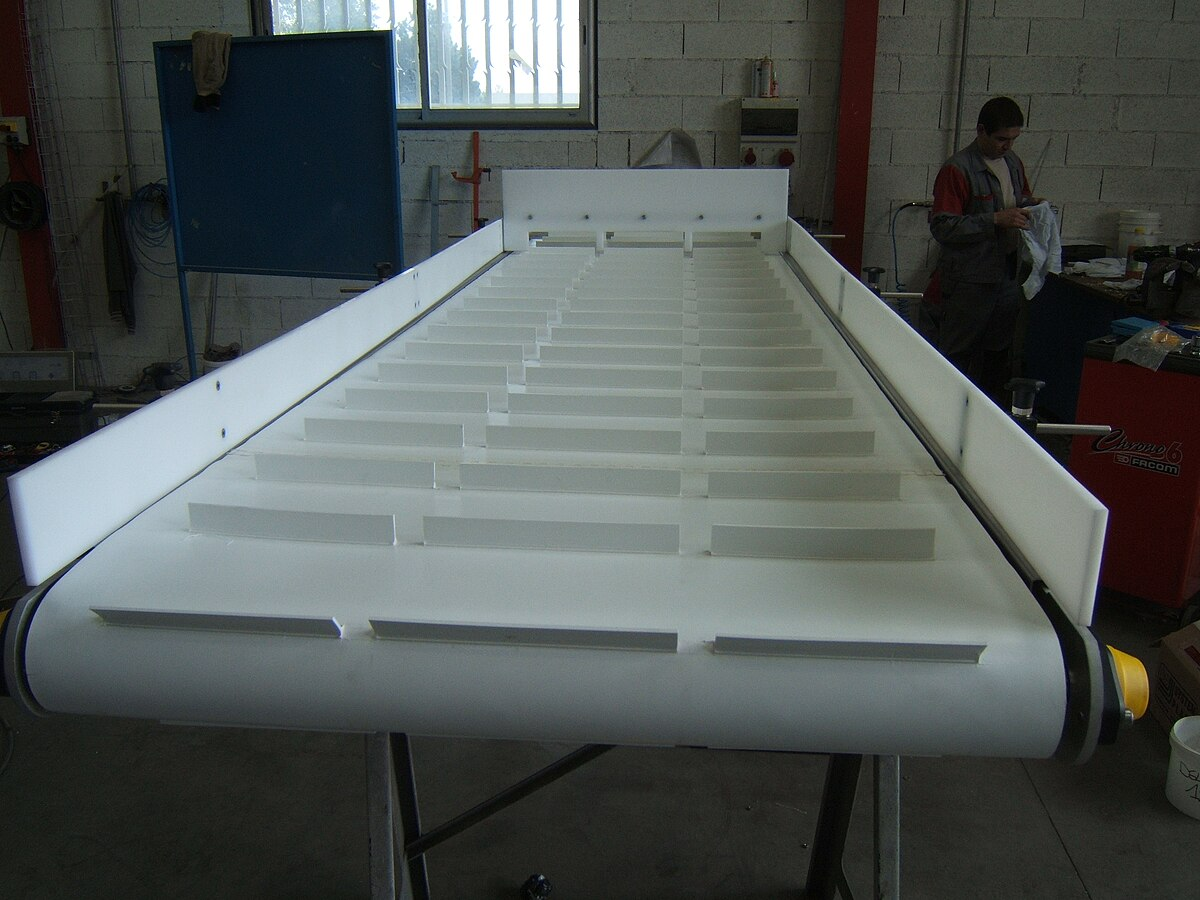
\includegraphics[width=\linewidth]{assets/figures/Hardware/transport_conv/convoyeur_tasseau.JPG}
        \caption{Convoyeur avec bande à tasseaux}
    \end{subfigure}\hfill
    \begin{subfigure}{0.45\textwidth}
        \centering
        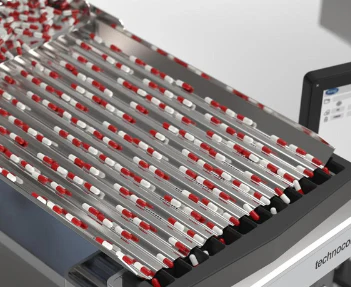
\includegraphics[width=\linewidth]{assets/figures/Hardware/transport_conv/convoyeur_tube.png}
        \caption{Convoyeur à tube}
    \end{subfigure}
    \caption{Convoyeurs}
\end{figure}

Quant aux différent moyen de movoir les capsules, il y a : 
\begin{itemize}
    \item les vibrations, 
    \item le déplacement de la bande, 
    \item la gravité.
\end{itemize}

La dernière option nécessite des surface lisse, que le système soit en pente et le temps de déplacement n'est pas réglable. Les deux autres solutions ne se distingue pas vraiment pour l'instant car dans tous les cas, l'utilisation d'un moteur électrique est nécessaire.

\subsection*{Déplacement à l'aide d'un robot}
Pour le déplacement des capsules, seul les axes $T_x, T_y~\text{et}~T_z$ sont nécessaires. Un robot de type \textit{SCARA}, cyclindrique ou Delta peuvent correspondre.

\subsection*{Avantanges et inconvénients}
\begin{table}[H]
    \caption{Anvantages et inconvénients des solution de saisie des capsules}
    \begin{tabular}{@{}cll@{}}
    \toprule
    Solution      & \multicolumn{1}{c}{Avantanges}                                                                                                   & \multicolumn{1}{c}{Inconvénient}                                                                                                                                  \\ \midrule
    Transport pneumatique par tube    & \begin{tabular}[c]{@{}l@{}}\end{tabular} & \begin{tabular}[c]{@{}l@{}}- Peu modulable\\ - Bruyant\\ - Aiguillage complexe\end{tabular}                                                                     \\
    Convoyeur & \begin{tabular}[c]{@{}l@{}}- \\ - \end{tabular} & \begin{tabular}[c]{@{}l@{}}- Maintenance fréquente\\ - Ne convient pas au petits objets\\ - Espace limité, pour pouvoir ouvrir \\ et fermer la pince \\ - Nécessite un contrôle de force\end{tabular} \\
    Robot   & \begin{tabular}[c]{@{}l@{}}- Place\\ - Modulable \\ \end{tabular}                            & \begin{tabular}[c]{@{}l@{}}- Coût\\ - Nécessite un nettoyage pour conserver \\  l'adhérence dans le temps\\ - Détachement complexe\end{tabular}     \\ \bottomrule
    \end{tabular}
\end{table}